%
%
\comment{
\begin{itemize}
	\item we need to do both width adaptation and clock-domain crossing
	\item draw out the schematic of FabricPort input/output
	\item how to determine VC? each message class has only one VC to choose from
	\item only one physical port can be connected to each FabricPort unless we can tolerate throughput degradation
	\item multiple VCs can still share the output mux ports to the fabric interconnect
\end{itemize}
}
%
%

This section describes the circuitry between our embedded NoC and the FPGA's fabric and I/Os.
The FabricPort is a flexible interface that connects to the FPGA fabric, and IOLinks are direct connections to I/O interfaces.

%
%---------------------------------------------------------------------------------------------------------
\subsection{FabricPort}
%---------------------------------------------------------------------------------------------------------
%

Each NoC port can sustain a maximum input bandwidth of 22.5~GB/s; however, this is done at the high frequency of 1.2~GHz for our NoC.
The main purpose of the FabricPort is therefore to give the FPGA fabric access to that communication bandwidth, at the range of frequencies at which FPGAs normally operate.
How does one connect a module configured from the FPGA fabric to the embedded NoC running at a different width and frequency?

%
\figvs{1}{fp_logical}{}{Data on the FPGA with any protocol can be translated into NoC flits using application-dependent soft logic (translator). A FabricPort adapts width (1-4 flits on fabric side and 1 flit on NoC) and frequency (any frequency on fabric side and 1.2~GHz on NoC side) to inject flits into the NoC.}
%

Fig.~\ref{fp_logical} illustrates the process of conditioning data from any FPGA module to NoC flits, and vice versa.
A very simple translator takes incoming data and appends to it the necessary flit control information.
For most cases, this translator consists only of wires that pack the data in the correct position and sets the valid/head/tail bits from constants.
Once data is formatted into flits, we can send between 0 and 4 flits in each fabric cycle, this is indicated by the valid bit on each flit.
The FabricPort will then serialize the flits, one after the other, and inject the valid ones into the NoC at the NoC's frequency.
When flits are received at the other end of the NoC, the frequency is again bridged, and the width adapted using a FabricPort; then a translator strips control bits and injects the data into the receiving module.

This FabricPort plays a pivotal role in adapting an embedded NoC to function on an FPGA.
We must bridge the width and frequency while making sure that the FabricPort is never a source of throughput reduction; furthermore, the FabricPort must be able to interface to different VCs on the NoC, send/receive different-length packets and respond to backpressure coming from either the NoC or FPGA fabric.
We enumerate the essential properties that this component must have:

\begin{enumerate}
\item \textbf{Rate Conversion}: Match the NoC bandwidth to the fabric bandwidth. Because the NoC is embedded, it can run \til4\xx faster than the FPGA fabric~\cite{trets}. We leverage that speed advantage to build a narrow-link-width NoC that connects to a wider but slower FPGA fabric.
\item \textbf{Stallability}: Accept/send data on every NoC cycle in the absence of stalls, and stall for the minimum number of cycles when the fabric/NoC isn't ready to send/receive data. The FabricPort itself should never be the source of throughput reduction.
\item \textbf{Virtual Channels}: Read/write data from/to multiple virtual channels in the NoC such that the FabricPort is never the cause for deadlock.
\item \textbf{Packet Length}: Transmit packets of different lengths.
\item \textbf{Backpressure Translation}: Convert credit-based flow-control into the more FPGA-familiar ready/valid.
\end{enumerate}


%
%\figvs{1}{stall_protocol}{}{Waveform of ready/valid signals between soft module $\rightarrow$ FabricPort input, or FabricPort output $\rightarrow$ soft module. After ``ready" signal becomes low, the receiver must accept one more cycle of valid data (data 2) after which the sender will have processed the ``ready" signal and stopped sending more valid data.}
%


\begin{figure*}[t]
\centering
\subfloat[FabricPort input: from the FPGA fabric to the embedded NoC.]{
   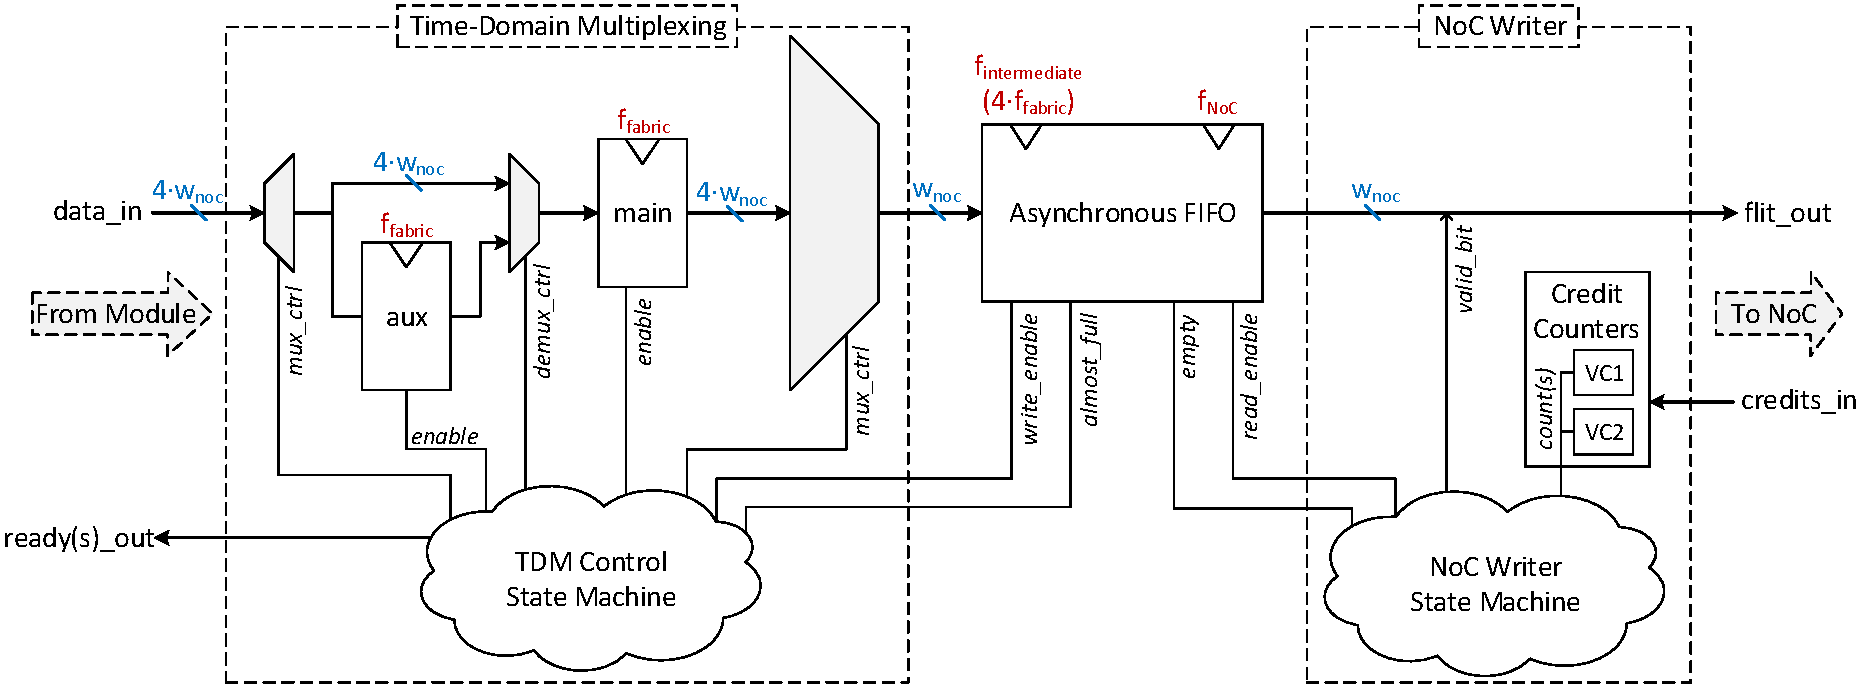
\includegraphics[width=2\columnwidth,keepaspectratio]{images/fpin_detail}
   \label{fpin}
 }
 \\
\subfloat[FabricPort output: from the embedded NoC to the FPGA fabric.]{
   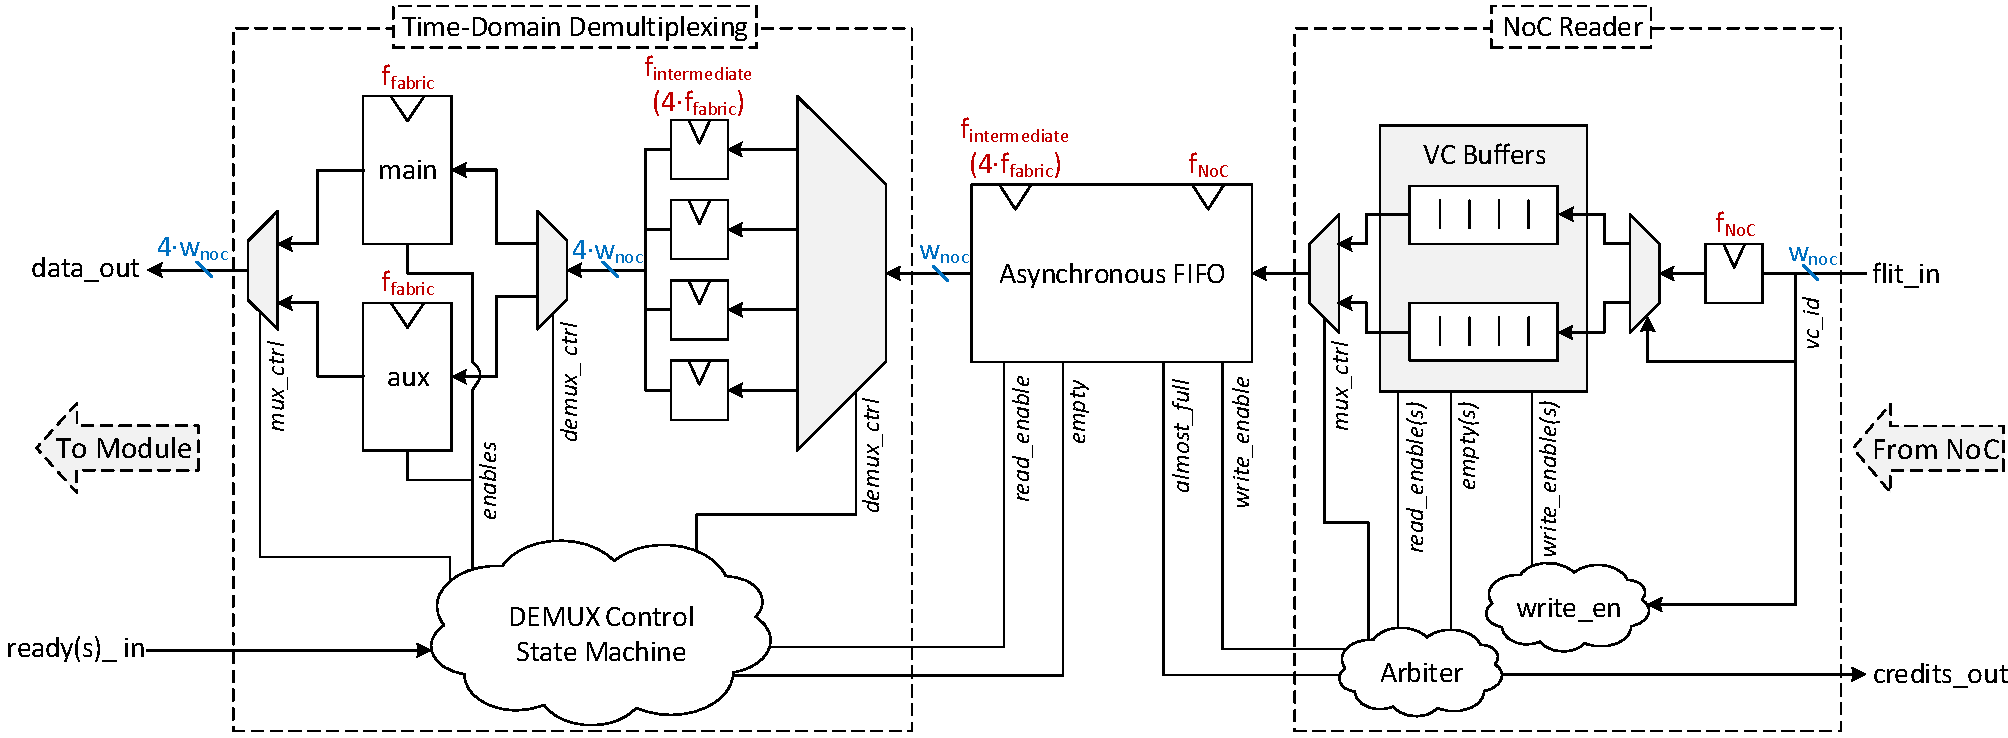
\includegraphics[width=2\columnwidth,keepaspectratio]{images/fpout_detail}
   \label{fpout}
 }
\caption{The FabricPort interfaces the FPGA fabric to an embedded NoC in a flexible way by bridging the different frequencies and widths as well as handling backpressure from both the FPGA fabric and the NoC.}
\label{fabric_port}
\end{figure*}

%----------------------------------------------------------------------------
\subsubsection{FabricPort Input: Fabric$\rightarrow$NoC}
%----------------------------------------------------------------------------

Fig.~\ref{fabric_port} shows a schematic of the FabricPort with important control signals annotated.
The FabricPort input (Fig.~\ref{fpin}) connects the output of a module in the FPGA fabric to an embedded NoC input.
Following the diagram from left to right: data is input to the time-domain multiplexing (TDM) circuitry on each fabric clock cycle and is buffered in the ``main" register.
The ``aux" register is added to provide elasticity. Whenever the output of the TDM must stall there is a clock cycle before the stall signal is processed by the fabric module.
In that cycle, the incoming datum may still be valid, and is therefore buffered in the ``aux" registers.
%To clarify this ready-valid behavior, example waveforms are illustrated in Fig.~\ref{stall_protocol}.
Importantly, this stall protocol ensures that every stall (ready = 0) cycle only stops the input for exactly one cycle ensuring that the FabricPort input does not reduce throughput.

The TDM unit takes four flits input on a slow fabric clock and outputs one flit at a time on a faster clock that is 4\xx as fast as the FPGA fabric -- we call this the intermediate clock.
This intermediate clock is only used in the FabricPort between the TDM unit and the asynchronous FIFO (aFIFO) buffer.
Because it is used only in this very localized region, this clock may be derived locally from the fabric clock by careful design of circuitry that multiplies the frequency of the clock by four.
This is better than generating 16 different clocks globally through phase-locked loops, then building a different clock tree for each router's intermediate clock (a viable but more costly alternative).

The output of the TDM unit is a new flit on each intermediate clock cycle.
Because each flit has a valid bit, only those flits that are valid will actually be written in the aFIFO thus ensuring that no invalid data propagates downstream, unnecessarily consuming power and bandwidth.
The aFIFO bridges the frequency between the intermediate clock and the NoC clock ensuring that the fabric clock can be completely independent from the NoC clock frequency and phase.

The final component in the FabricPort input is the ``NoC Writer".
This unit reads flits from the aFIFO and writes them to the downstream NoC router.
The NoC Writer keeps track of the number of credits in the downstream router to interface to the credit-based backpressure system in the embedded NoC, and only sends flits when there are available credits.
Note that credit-based flow control is by far the most-widely-used backpressure mechanism in NoCs because of its superior performance with limited buffering~\cite{dally_book}.
%Each sender keeps count of the number of credits; the sender has a credit for each available downstream buffer location.
%Therefore, a sender will only send data if it has available credits (telling it that there is buffer space downstream).
%The downstream buffer sends a credit upstream only when it has freed one of its buffer locations by forwarding a flit.

%
%----------------------------------------------------------------------------
\subsubsection{FabricPort Output: NoC$\rightarrow$Fabric}
%----------------------------------------------------------------------------
%

Fig.~\ref{fpout} details a FabricPort output; the connection from an NoC output port to the input of a module on the FPGA fabric.
Following the diagram from right to left: the first component is the ``NoC Reader".
This unit is responsible for reading flits from an NoC router output port and writing to the aFIFO.
Note that separate FIFO queues must be kept for each VC; this is very important as it avoids scrambling data from two packets.
Fig.~\ref{demux} clarifies this point; the upstream router may interleave flits from different packets if they are on different VCs.
By maintaining separate queues in the NoC reader, we can rearrange flits such that flits of the same packet are organized one after the other.

The NoC reader is then responsible for arbitrating between the FIFO queues and forwarding one (entire) packet -- one flit at a time -- from each VC.
We currently implement fair round-robin arbitration and make sure that there are no ``dead" arbitration cycles.
That means that as soon as the NoC reader sees a tail flit of one packet, it has already computed the VC from which it will read next.
The packet then enters the aFIFO where it crosses clock domains between the NoC clock and the intermediate clock.

The final step in the FabricPort output is the time-domain demultiplexing (DEMUX).
This unit reassembles packets (or packet fragments if a packet is longer than 4 flits) by combining 1-4 flits into the wide output port.
In doing so, the DEMUX does not combine flits of different packets and will instead insert invalid zero flits to pad the end of a packet that doesn't have a number of flits divisible by 4 (see Fig.~\ref{demux}).
%This is very much necessary to simplify the output of the NoC into something that is understandable by designers thereby creating an abstracted view of the NoC without complicating design.
This is very much necessary to present a simple interface for designers allowing them to connect design modules to the FabricPort with minimal soft logic.


%
\figvs{1}{demux}{}{``NoC Reader" sorts flits from each VC into a separate queue thereby ensuring that flits of each packet are contiguous. The DEMUX then packs up to four flits together and writes them to the wide output port but never mixes flits of two packets.}
%



%
%---------------------------------------------------------------------------------------------------------
\subsection{IOLinks}
%---------------------------------------------------------------------------------------------------------
%


The FabricPort interfaces between the NoC and the FPGA in a flexible way.
To connect to I/O interfaces, such as external memory interfaces, we can connect through a regular Fabricport interface.
This could be done by simply connecting the I/O interface to soft logic which then connects to a FabricPort as shown in Fig.~\ref{io_fp}.
However, the soft logic between an I/O interface and the FabricPort may be difficult to design for many reasons:

%
\begin{itemize}
    \item Fast I/O interfaces have very stringent timing requirements, making timing closure on any soft logic connecting to it very challenging.
    \item The NoC router may be physically placed far away from the I/O interface, thus heavily-pipelined soft logic is required to connect the two. This may incur significant area and power overhead as the data bandwidth of some I/O interfaces is very large, which translates into a wide data path in the slow FPGA logic. Furthermore, adding pipeline registers would improve timing but typically worsen latency -- a critical parameter of transferring data over some I/Os.
    \item Any solution is specific to a certain FPGA device and will not be portable to another device architecture.
\end{itemize}
%

%
\begin{figure}[t]
\centering
\subfloat[Through the FabricPort.]{
   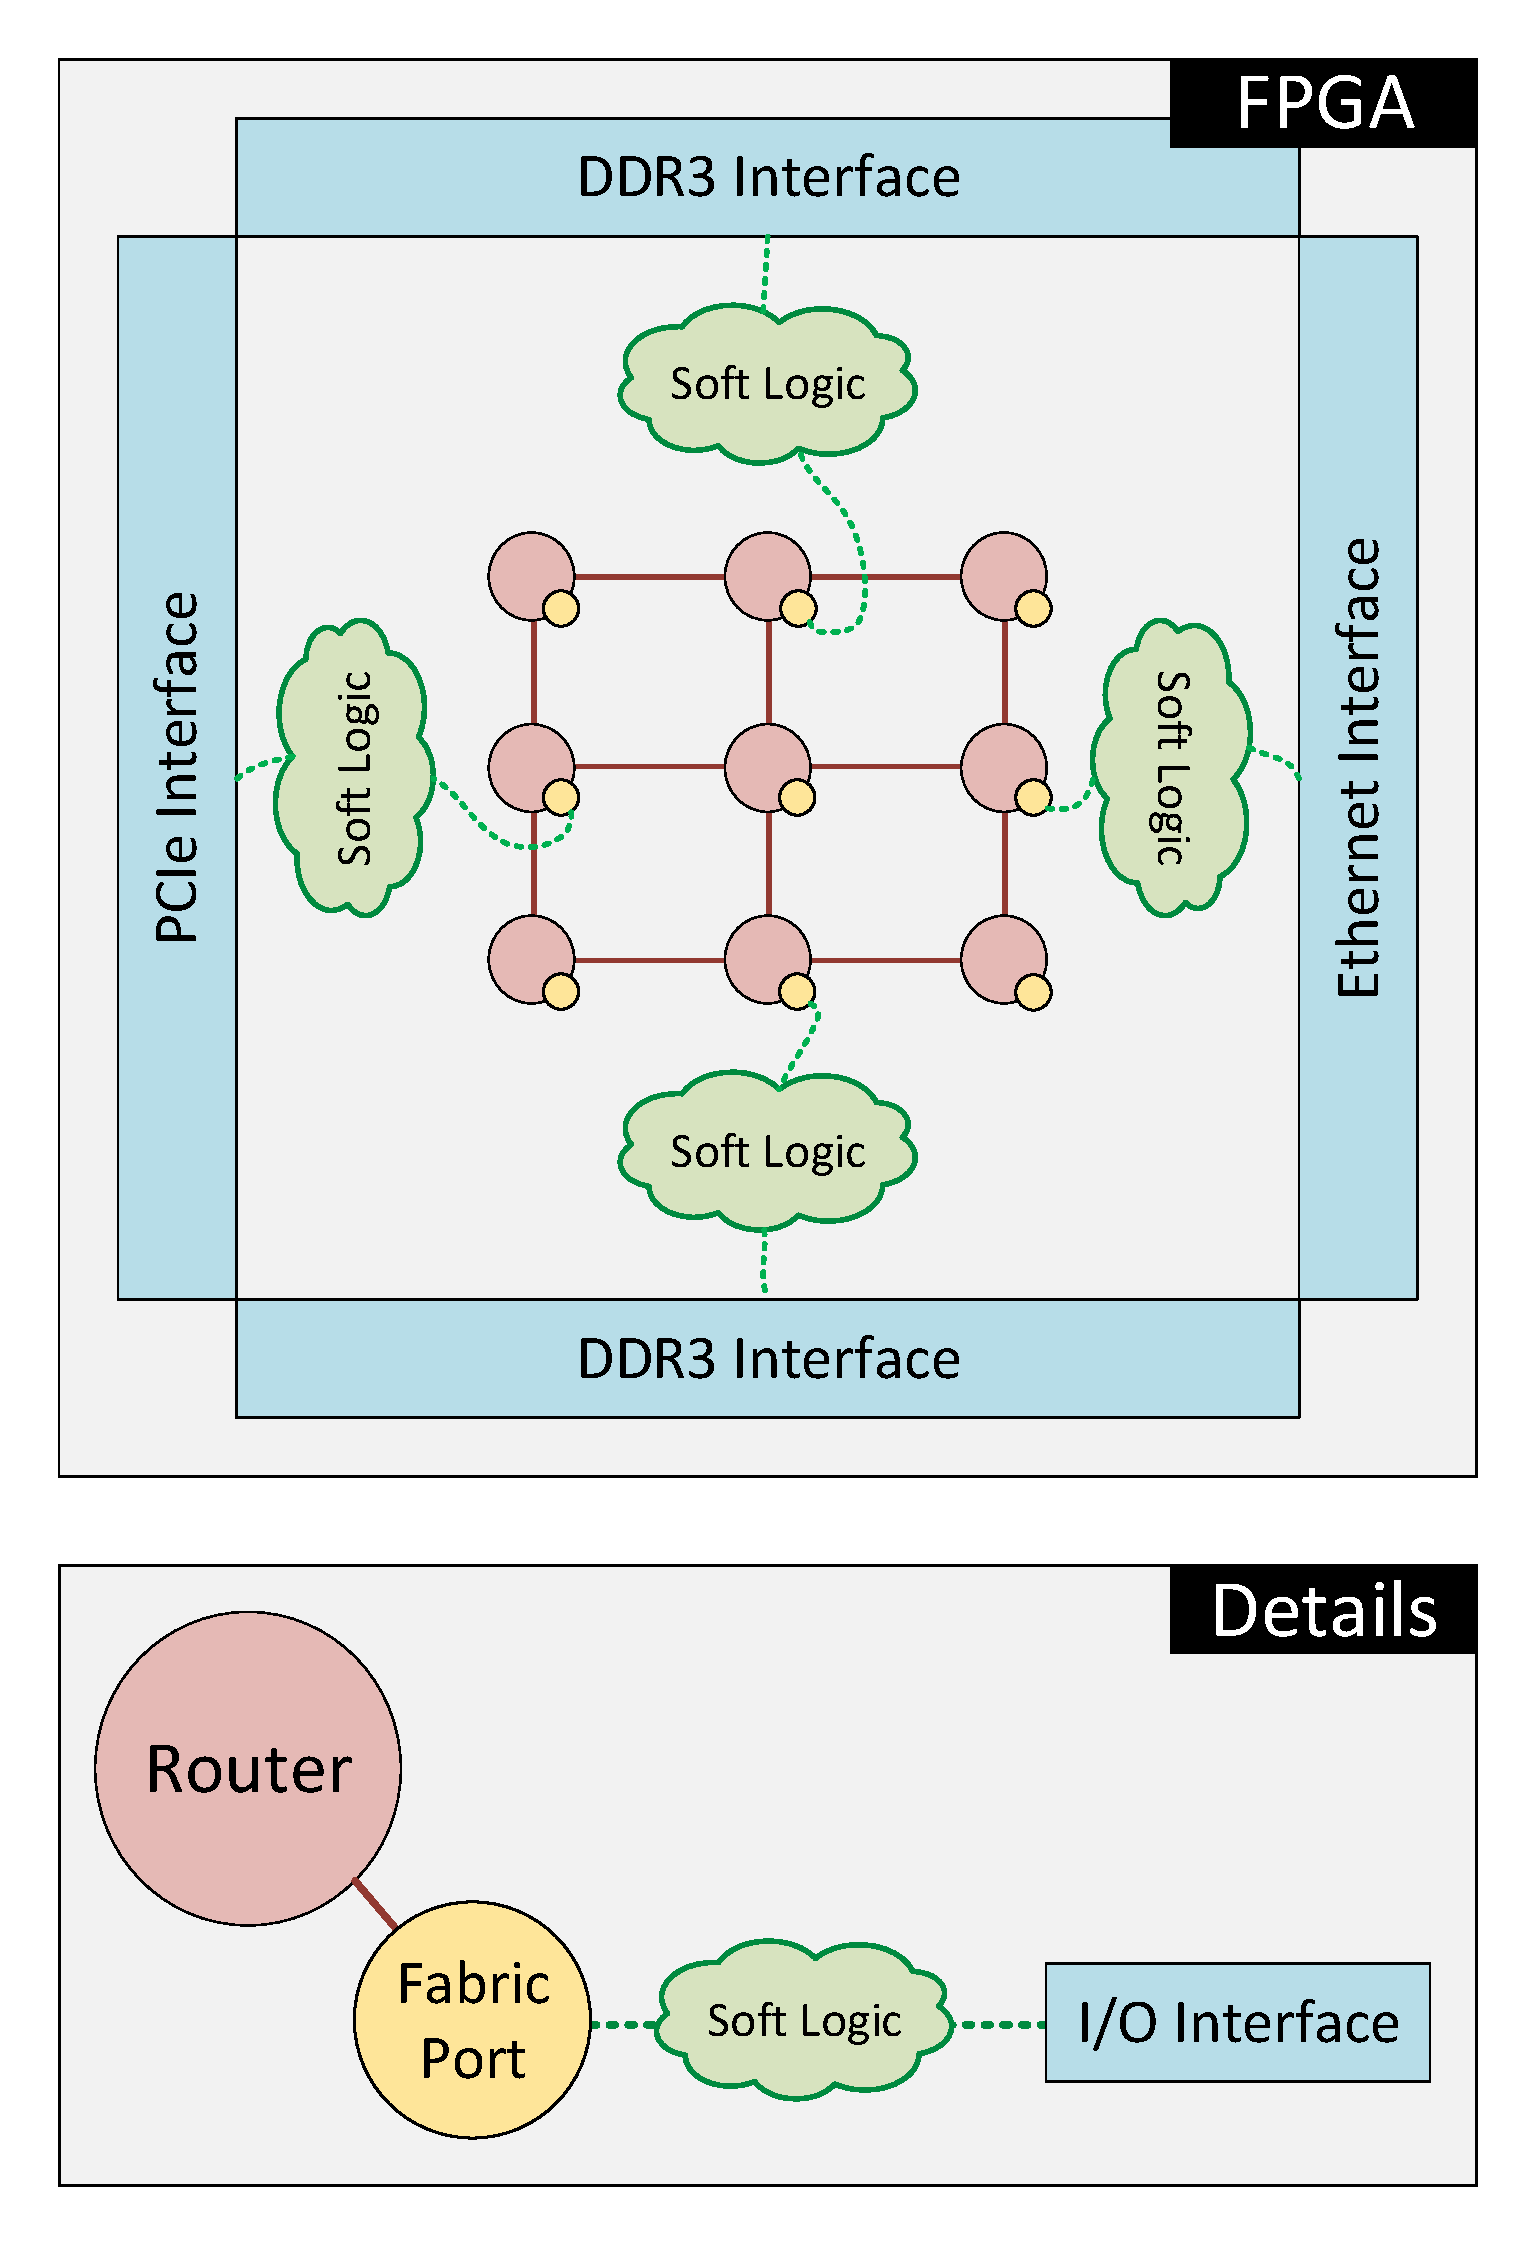
\includegraphics[width=0.49\columnwidth,keepaspectratio, trim = 0cm 0cm 0cm 2.3cm]{images/io_direct}
   \label{io_fp}
 }
\subfloat[Directly using hard IOLinks.]{
   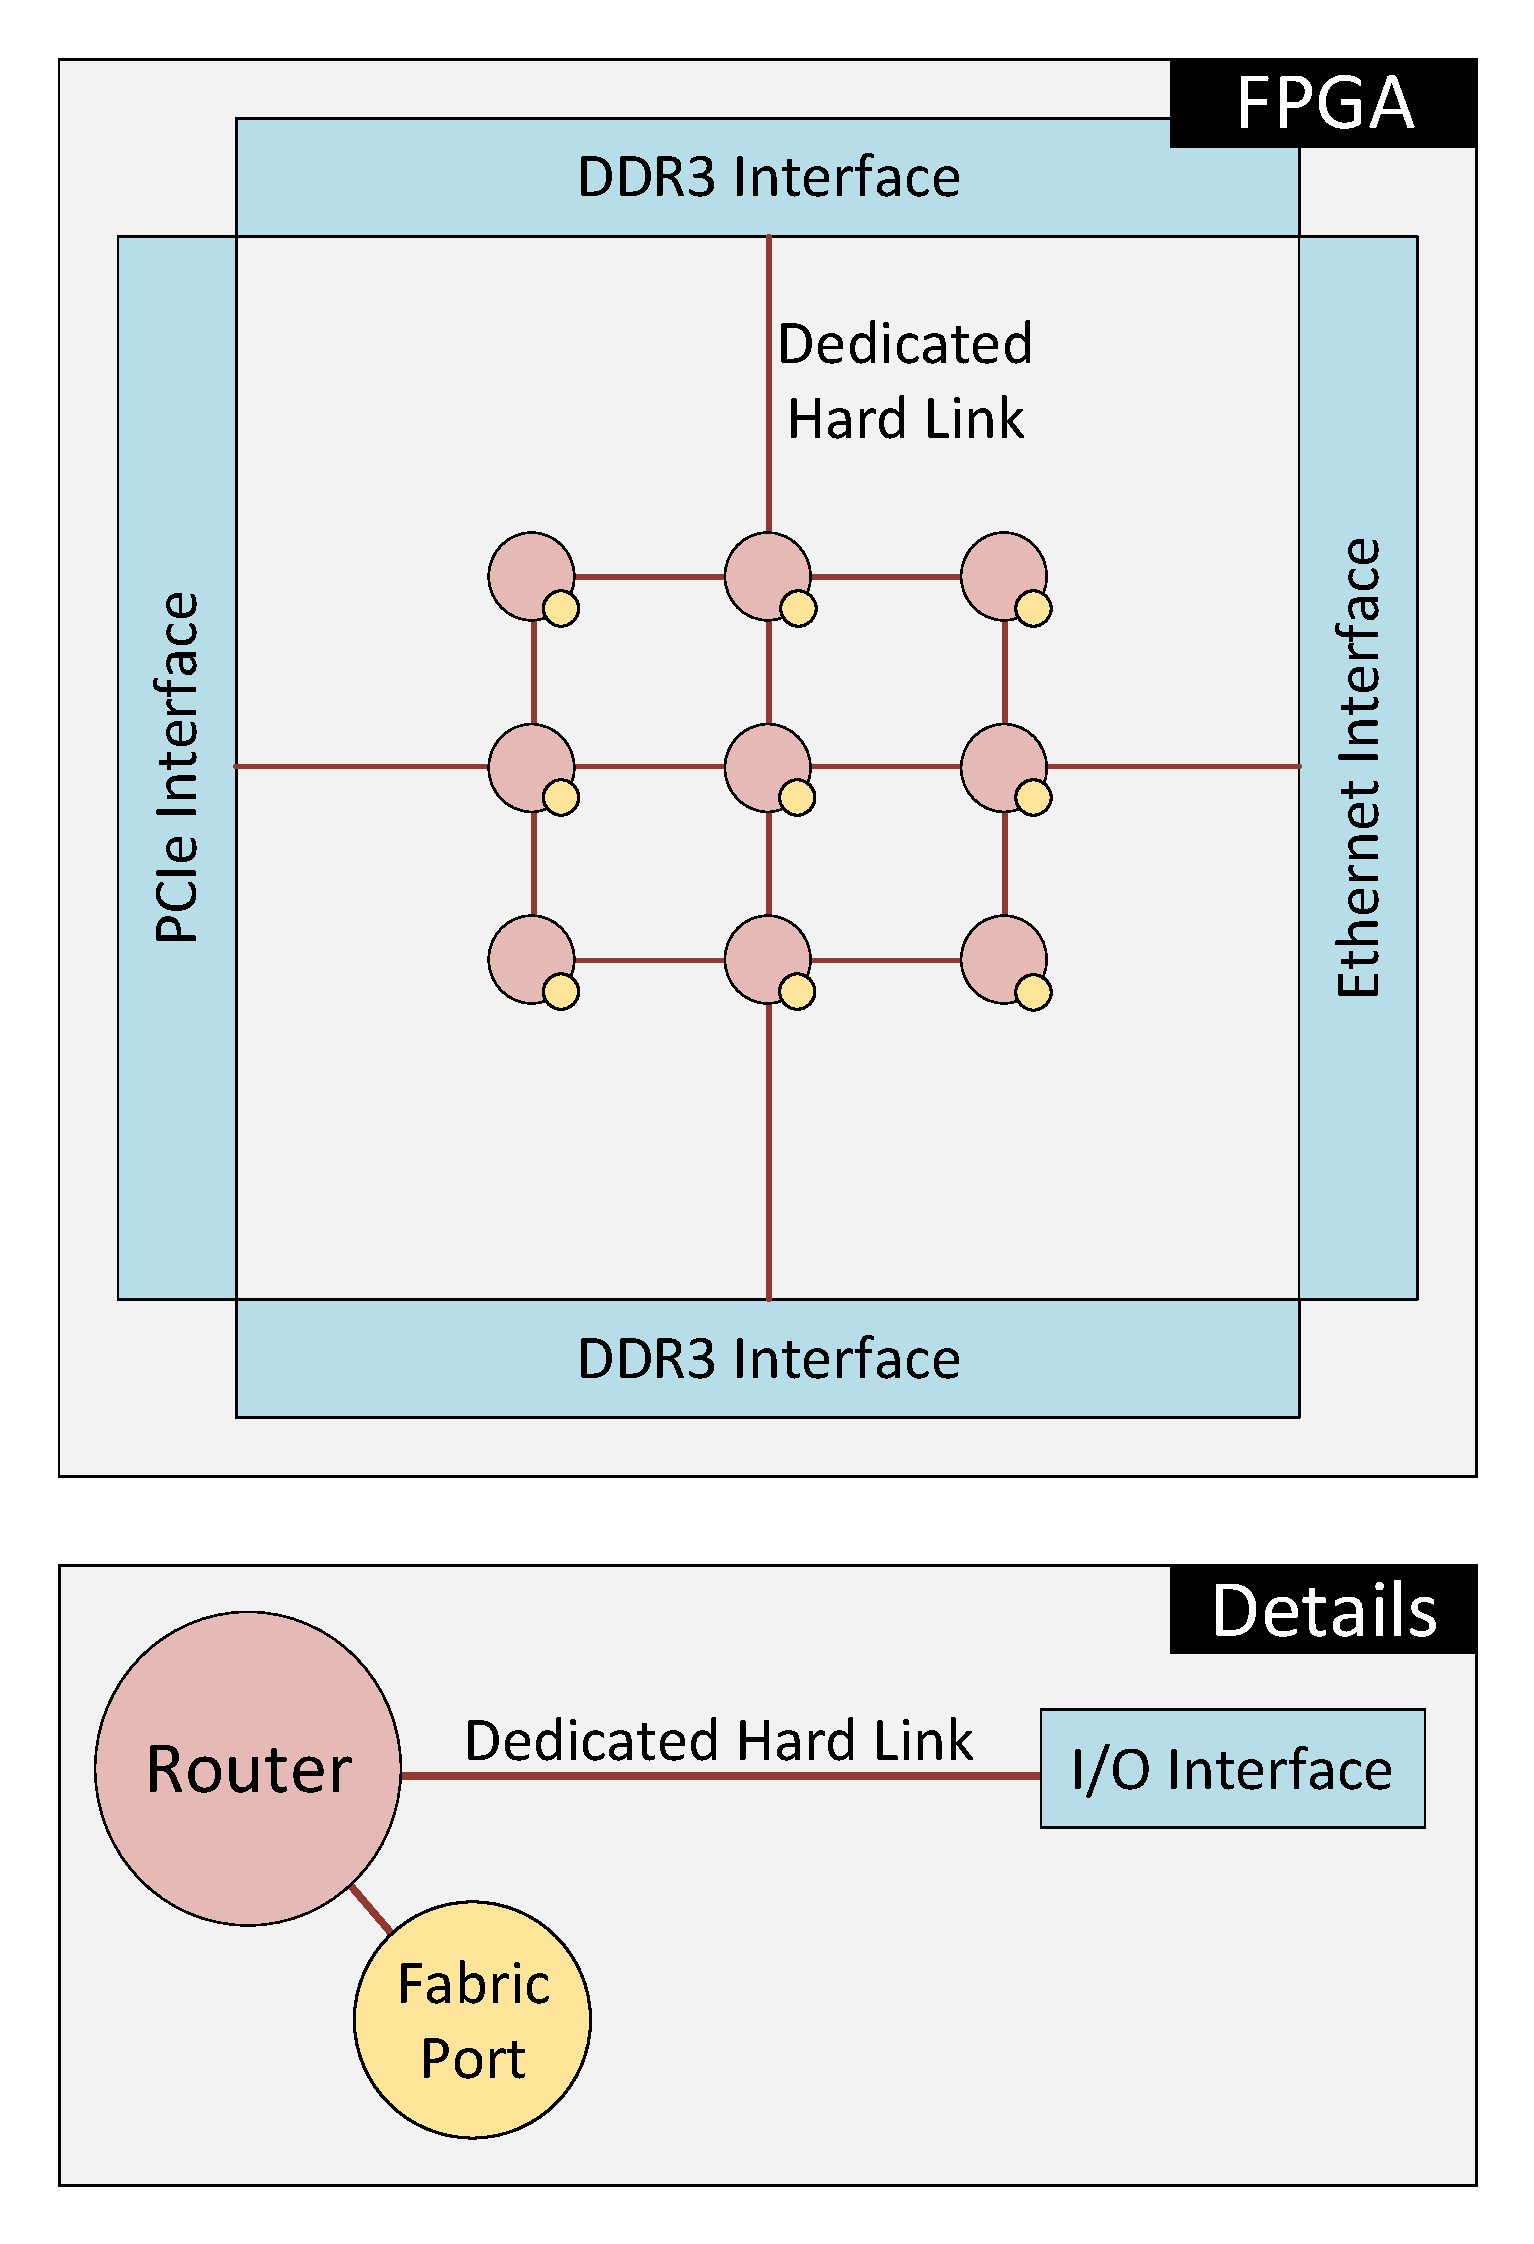
\includegraphics[width=0.49\columnwidth,keepaspectratio, trim = 0cm 0cm 0cm 2.3cm]{images/io_fp}
   \label{io_direct}
 }
\caption{Two options for connecting NoC to I/O interfaces.}
\label{two_options_io}
\end{figure}
%

These shortcomings are the same ones that we use to motivate the use of an embedded NoC instead of a soft bus to distribute I/O data.
Therefore, if we connect to I/O interfaces through the FabricPort, we lose some of the advantages of embedding a system-level NoC.
Instead, we propose connecting NoC routers directly to I/O interfaces using hard links as shown in Fig.~\ref{io_direct}.
In addition, clock-crossing circuitry (such as an aFIFO) will be required to bridge the frequency of the I/O interface and the embedded NoC since they will very likely differ.
We call these direct I/O links with clock crossing ``IOLinks".
They have many advantages:

%
\begin{itemize}
    \item Uses fewer NoC resources since it frees a FabricPort which can be used for something else.
    \item Reduces soft logic utilization conserving area and power.
    \item Reduces data transfer latency between NoC and I/O interfaces because we avoid adding pipelined soft logic.
\end{itemize}
%

One possible shortcoming of IOLinks is the loss of reconfigurability -- it is important to design these I/O links such that they do not rid the FPGA I/O interfaces of any of their built-in flexibility.
IOLinks should be optional by using multiplexers in the I/O interfaces to choose between our IOLinks and the traditional interface to the FPGA logic.
This will maintain the option of directly using I/O interfaces without using IOLinks, thus maintaining the configurability of I/O interfaces.
Note that an IOLink's implementation will be very specific to the I/O interface to which it connects; we study an IOLink to DDR3 interface in Section~\ref{sec_ddr}.

\comment{
To be able to send packets to the directly-connected I/O interfaces, we need to extend NoC addressing to include the directly-connected I/Os.
For example, our proposed NoC has 16 routers and therefore requires 4 addressing bits in its packet format.
However, this NoC can connect up to 16 I/O interfaces along its perimeter (by extending the mesh topology at each side).
We therefore have a maximum of 32 different addresses (16 routers and 16 direct I/Os) for this NoC and we will require 5 address bits instead of 4.
}
%
%
